\documentclass[draftclsnofoot, onecolumn, letterpaper,10pt,compsoc]{IEEEtran}

\usepackage{url}
\usepackage{color}
\usepackage{hyperref}
\hypersetup{
    colorlinks=true,
    linkcolor=blue,
    filecolor=magenta,      
    urlcolor=blue,
}
\usepackage{geometry}
\usepackage{tabularx}
\usepackage{listings}
\usepackage{fancyvrb}
\usepackage{varwidth}
\usepackage{setspace}
\usepackage{float}
\usepackage{caption}
\usepackage{graphicx}
\usepackage{pgfgantt}
\graphicspath{ {./images/} }

\geometry{margin=0.75in}   
\singlespacing

\def \TitlePageHeader{Droplet Productions}
\def \TitlePageTitle{Progress Report}
\def \GroupNumber{by Group 13}
\def \GroupMembers{James Barry, Tarren Engberg, Dennis Li, James Luo,  Brice Ng}
\def \CourseTitle{CS 462 - Senior Design}
\def \CourseTerm{Winter 2018}

\title{Group13ProgressReport}
			
\newcommand{\NameSigPair}[1]{\par
\makebox[2.75in][r]{#1} \hfil 	\makebox[3.25in]{\makebox[2.25in]{\hrulefill} \hfill		\makebox[.75in]{\hrulefill}}
\par\vspace{-12pt} \textit{\tiny\noindent
\makebox[2.75in]{} \hfil		\makebox[3.25in]{\makebox[2.25in][r]{Signature} \hfill	\makebox[.75in][r]{Date}}}}
\renewcommand{\NameSigPair}[1]{#1}


%i pull \centerfloat from memoir here, so i can use it for figures
\makeatletter
\newcommand*{\centerfloat}{%
  \parindent \z@
  \leftskip \z@ \@plus 1fil \@minus \textwidth
  \rightskip\leftskip
  \parfillskip \z@skip}
\makeatother


\begin{document}
\begin{titlepage}
    \pagenumbering{gobble}
    \begin{singlespace}
        \hfill    
        \par\vspace{.2in}
        \centering
        \scshape{
            \huge \TitlePageHeader \par
            {\large\today}\par
            \vspace{.5in}
            \textbf{\Huge \TitlePageTitle }\par
            \vfill
            \vspace{5pt}

            \vspace{5pt}
            {\Large
                \NameSigPair{\GroupNumber}\par
            	\NameSigPair{\GroupMembers}\par
                \NameSigPair{\CourseTitle}\par
                \NameSigPair{\CourseTerm}\par
            }
            \vspace{20pt}
        }
    \end{singlespace}
    \begin{abstract}
    This document is a review of Group 13's progress in developing Droplet during Winter term. The document includes a recap of the project's purpose, a report on the Group's current progress, an overview of the remaining work, and a description of the problems encountered during development along with their respective solutions, if any.
    \end{abstract}
\end{titlepage}

\newpage
\pagenumbering{arabic}
\clearpage

\pagebreak

\section{Project Purposes and Goals Recap}
The project is a location-tagging mobile application called Droplet. Its goal is to bring physical connection to social media by making people explore the world to see posts made by others. The project attempts to achieve this goal by attaching a user's posts to a location instead of just to their account. In addition, only nearby users can view and interact with those posts. By limiting interactions to posts made within someone's general vicinity, it filters out information that a user cannot physically interact with while encouraging users to actively search for posts via exploration.

\section{Current Progress}
\subsection{Database}
The team has created a testing MongoDB server using an automated cloud service, and has successfully connected to the database.  In addition, back-end endpoints have been created for post and comment CRUD (Create, Read, Update, and Delete) functionality.  Posts have the option of being text, a picture, or a combination of both.  Database maintenance includes storing pictures in a local folder to minimize data stored on the database, and deleting the comments of a deleted post to minimize floating data.  Below is a snippit of code from the post schema Droplet has implemented.  This schema details what information the post will consist of, and what types the fields accept.

\begin{lstlisting}
const postSchema = new mongoose.Schema({
    _id: mongoose.Schema.Types.ObjectId,
    username: {
        type: String,
        ref: 'User',
        required: 'Username is required'
    },
    content: {
        type: String
    },
    postImage: {
        type: String,
        default: undefined
    },
    comments: [{
        type: mongoose.Schema.Types.ObjectId,
        ref: 'Comment',
        required: 'Comment is required'
    }],
    created: {
        type: Date,
        default: Date.now
    },
    updated: {
        type: Date,
        default: Date.now
    },
//    location: {
//        latitude: Number,
//        longitude: Number,
//        default: undefined
//    },
    likes: [{
        type: mongoose.Schema.Types.ObjectId,
        ref: 'User'
    }]
});
\end{lstlisting}

The back-end currently allows for users to be created, each with a unique username, a hashed password, and an automatically generated unique ID.  These users can create posts, with each post structured as above.  The location field is currently commented out due to not having the permissions to access IP location implemented.  As seen above, each post has a comment array to be filled with ID's of comments and a likes array to be filled with userID's of users who liked the post.  Below is the code used to like a post.
\begin{lstlisting}
//Check if user has already liked the post
    Post.find( { "_id" : Pid, likes: {$in: [Uid] }  }, (err, post) => {
        if(err) {
            return res.status(500).send(err);
        }
        //Already liked the post
        else if(post.length > 0 ) {
            return res.status(401).json({
                success: "You have already liked this post!"
            });
         }
        else {
            //Like the post
            Post.updateOne({ "_id" : Pid}, {$push: { likes: Uid}}, (err, post) => {
                if(err) {
                    return res.status(500).send(err);
                }
                else {
                    return res.status(200).json({
                        success: 'You have liked this post!'
                    });
                }
            });
        }
    });
\end{lstlisting}
This first checks to see if a user has already liked a post by checking to see if the username is in the 'like' array.  If they have, then they cannot duplicate the like.  If the username is not in the array, then it is appended to the end and the array is updated.  Every other scenario generates an appropriate error.

\subsection{Map}
The team has implemented a Map into the application using the MapBox API. Currently, they are able to display a basic Map onto the screen. This Map allows users to click and drag to various locations on the Map, and zoom into a specific location. In addition to displaying a Map, our team has successfully added markers onto the Map at distinct points with their longitude and latitudes. The marker icon has also been changed to the droplet icon to match our initial mock-ups. Currently, the style of the Map is very simple, but aesthetically pleasing for users.

\begin{figure}[!ht]
    \centering
    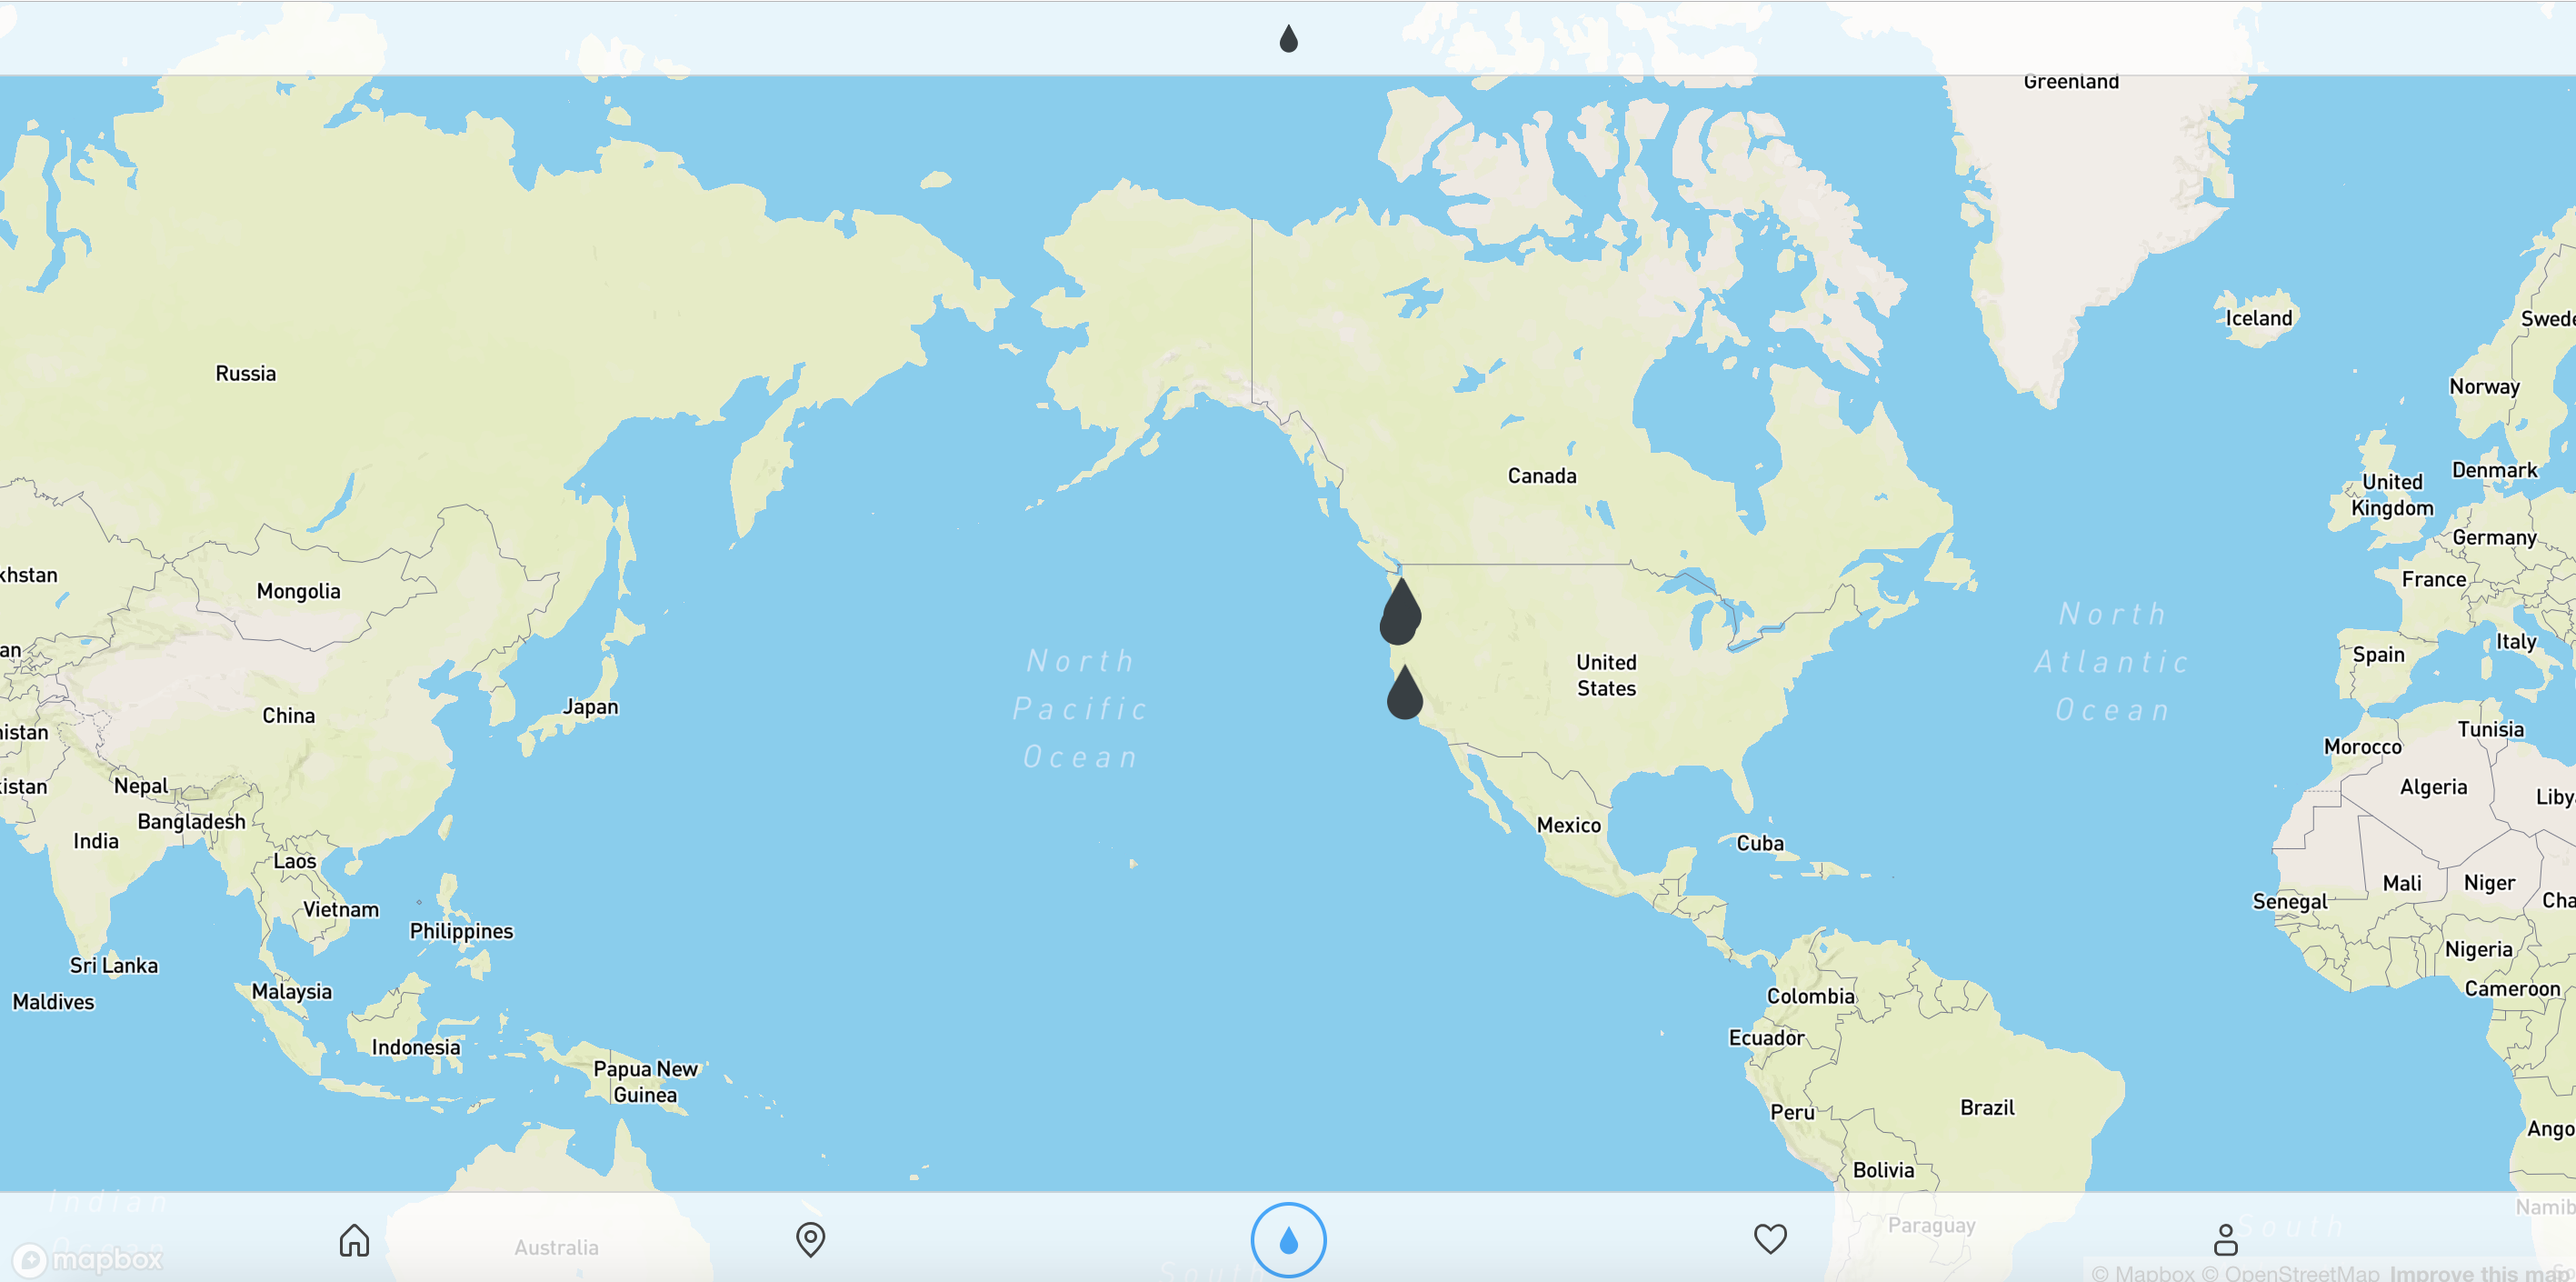
\includegraphics[scale=.25]{images/Map1.png}
    \caption{Map Screen Zoomed Out}
    \label{fig:my_label}
\end{figure}
\begin{figure}[!ht]
    \centering
    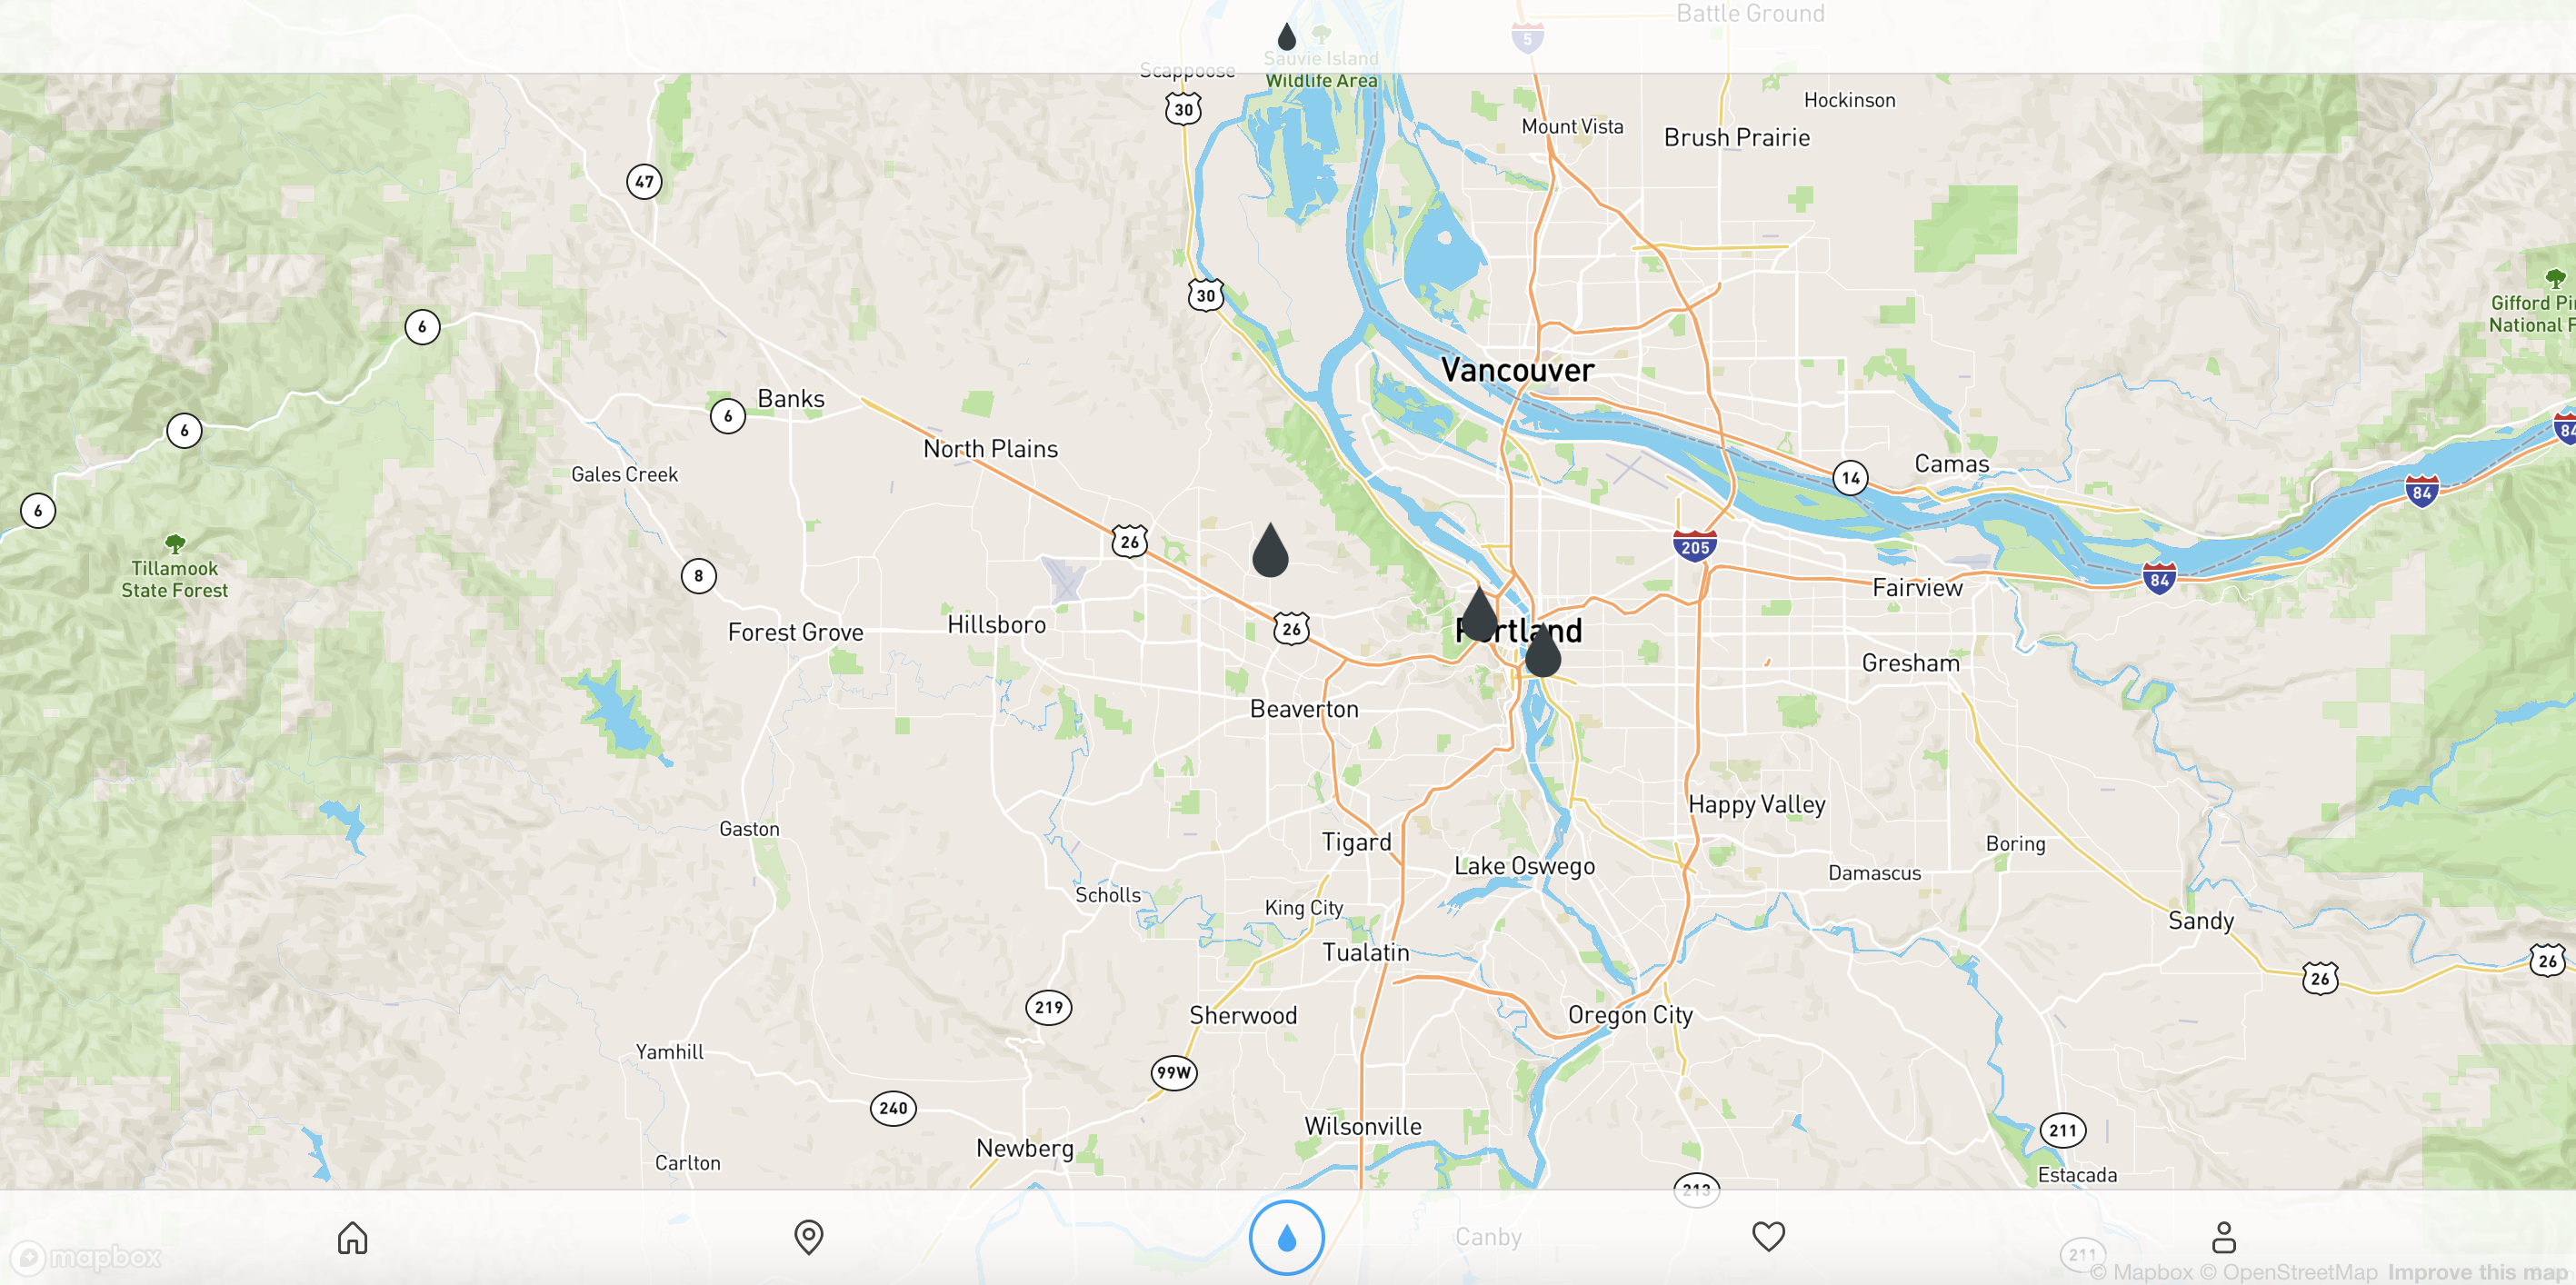
\includegraphics[scale=.25]{images/Map2.png}
    \caption{Map Screen Zoomed In}
    \label{fig:my_label}
\end{figure}

\pagebreak

\subsection{Authentication}
The team has opted to use JSON Web Tokens (JWTs) to handle user authentication, and currently there is a basic login page that is capable of parsing the user's inputs and storing them in the state. It's been linked to the back-end, allowing it to send the username and password to an existing database and receive a response back.

\subsection{Other Client Screens}
The team has managed to integrate the Redux client library to simplify the app state management and enforce a system for subscribing to app state changes that is immutable and functionally scalable. The home page is able to asynchronously fetch post data from the server and display their content in list view. Recent changes have included a reorganization of the navigation hierarchy to make the first three pages, which all have the same dynamic map background, to be considered the home page, with the three sub-pages of posts, map-only view and the new-post view. The new-post page is in progress and still under construction.

\section{Remaining Work}
\subsection{Database}
%The back-end currently was made without keeping track of users in mind.  It needs to be refactored with a user schema in place so that postId's are connected to a user, likewise with comments.  The appropriate endpoints will also need to be corrected to incorporate the new schema.  Comments are also missing Update functionality, and the endpoints are not connected to the front-end as of yet.
Currently, the back-end has user, post and comment CRUD functionality.  The remaining back-end work that needs to be done is accept location information from the device, ideally the longitude and latitude, and implement the location field.  When the map is fully integrated, the team will need to determine how extract the information and use it meaningfully.  It should be noted that the back-end is not connected to the front-end aside from user authentication, and that the team is currently working on integrating the two. 

\subsection{Map}
In the end, the team wants to be able to view posts near users from the map. Currently, the Map is not interactive besides being able to drag and zoom the map. The team also wants to be able to add popups that show the posts. In order to implement this we would need to be able to create the popups and connect it with the data from the database. In regards to the style, if the team decides to change the style, the team can implement this through using MapBox API's present styles. In addition, a new style can be created through MapBox Web Studio and integrated into the application. The final aspect we would need to add to our application is requesting user location for the map.

\subsection{Authentication}
There isn't currently any button for logging in, since it's still up in the air exactly how to go about asking the user to login (a small popup, a unique window, should the user be asked to login when they start the app/page, etc.) In addition, although a user can technically login and receive a JWT, the application doesn't use the JWT for anything at the moment, so anyone can still access anything and being "logged in" doesn't actually mean anything. The UI doesn't update itself to reflect that a user is logged in either (i.e. when logged in, there should be a logout button). 

\subsection{Other}
In addition to the work listed above, there are various elements that still need to be implemented. A page or popup for creating posts still needs to be made, and it will have to be linked to the back-end and send things such as post content and location data to the database. Interacting with posts themselves (not on the map) still needs to be worked on too i.e. comments and likes. 

\section{Problems and Solutions}

\subsection{The Big Data Problem}
An ongoing point of discussion for the group has been how to store and parse information. Since posts are based on locations, they're spattered around in an unstructured way. Organizing these is important, because, as the size of our database approaches infinity, it becomes gradually more time consuming to search the database for posts that are nearby the user. 

A simple way that lends itself to MongoDB's structure would be to nest posts within the user that posted them, and then nest comments for each post within the post. This means, if you want all the posts associated with a particular user, you just ask the database for the user; no searching is required. However, given that getting posts that are nearby the current user is top priority, having them organized this way would be very inefficient. The entire database would need to be searched to get posts nearby the user, since they're not sorted by location. 

Our first idea for solving this issue was to split the world into sectors. Posts would be organized into their respective sectors. Then, when a user asks for posts nearby, their current sector and all adjacent sectors would be checked for posts. However, the question then become as follows: How small do we need to make the sectors to avoid the infinity problem? Would we have an efficient way to subdivide sectors if a given sector gets too full?  Because of these issues, we brainstormed more.

Our second idea was to sort posts in the database based on their latitude. Then, when a user asks for posts, we "create" a sector for the part of the earth they're in on the fly and only return posts in that sector. However, math for that is complex and time consuming (see next section). An alternate version of this, suggested by our TA Chris, would be to store each post with a "real" lat/long pair and a "search" lat/long pair. The "real" pair would be as specific as possible, while the "search" pair would only be accurate down to the half latitude/longitude degree. Then, when we ask the database for posts, we base the search on the "search" pair, so that specificity doesn't slow down the search. Then, any desired geographical maths could be performed on this subset of data to reduce time required. 

We're focusing on that final solution for now. At the end of the day, if that doesn't work out and we can go with something simpler but slower, we will. In the current phase of development we just need something that works. 

\subsection{Great Circle Navigation}

An issue in our effort to make database parsing efficient is that calculating the distance between two points on a sphere is difficult. This arises from how \href{https://en.wikipedia.org/wiki/Geographic_coordinate_system}{geographic coordinate systems} work. The idea of latitude and longitude is common knowledge, but some of the fine details are not-so-common, so here's a breakdown. 

\begin{itemize}
    \item Great circle navigation is the study of travelling across a spherical object, which has many implications in long-distance nautical and air travel.
    \item Geographic coordinate systems are methods for quantifying where a given location on a sphere is, typically a doublet (horizontal, vertical) or a triplet (horizontal, vertical, elevation).
    \item Latitude, longitude, and elevation is a popular geographic coordinate system choice. We care about latitude and longitude. 
    \begin{itemize}
        \item Latitude is a measure of horizontal position. Each degree of latitude at a given longitude is the same size as any other degree of latitude at that same longitude. 
        \item Longitude is a measure of vertical position. Each degree of longitude becomes progressively smaller than the last as distance from the equator increases. 
    \end{itemize}
\end{itemize}

Some of the complexities may come through based on those descriptions. Let's highlight a few. 

First, the size of a given latitude degree is a function of the longitude it is at. Think of it this way: take a cross section at the Earth's equator and measure its circumference, and then take a cross section (in the same direction as the last) near one of the poles and measure its circumference. A full circle of latitude goes around both of these cross sections, but each circumference is a different size, so the meters-distance represented by each circle is different. 

\begin{figure}[H]
    \centerfloat
    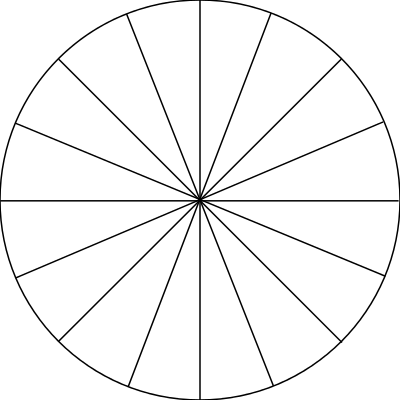
\includegraphics[scale=.5]{images/latitude.png}
    \caption{Points of latitude radiate circularly from the center axis. The distance represented by each degree is equal.}
\end{figure}

Second, each degree of longitude represents a gradually smaller meters-distance as distance from the equator increases. This is because of how the two are measured. 

\begin{figure}[H]
    \centerfloat
    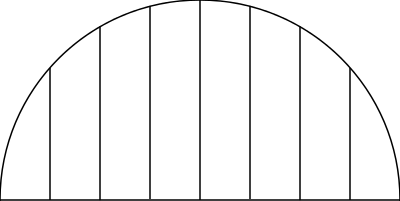
\includegraphics[scale=.5]{images/longitude.png}
    \caption{Points of longitude extend parallel to each other. The distance represented by each degree varies based on distance from the equator.}
\end{figure}

As such, formulas for calculating distance between two geographical coordinates are rather dense. The \href{https://en.wikipedia.org/wiki/Haversine_formula}{Haversine formula}, which first arose in 1801, is fairly complicated. If we want to know what posts are within a certain meters-distance from the user, it's not as simple as it may sound.  This is all just to say that our difficulties with Big Data described in the previous section become considerably more difficult when these issues are also considered. 
%The team has encountered a problem when deciding how to parse information on a global scale. The problem is that, because of Earth's curvature, longitude is not a consistent unit of measurement. To handle this, the team has been researching the haversine formula to convert longitude and latitude to meters. This is needed since user's should be able to set the "splash radius" of their posts, and asking them to do so using latitude and longitude would be impractical. 


%There's also a problem with the storage of posts. The team originally planned to have posts be a part of a user, but given that Droplet is meant to focus more on locations, this changed to having all posts stored in one giant list. However upon further thought, it was concluded that doing so could cause long delays when searching for "nearby" posts. One potential solution involved splitting the world into zones, where only the current and adjacent zones (to account for cases where the user or a post was near the edge of a zone) would be searched. Another alternative was to simply keep the list sorted at all times based on latitude and longitude, thereby allowing the use of more efficient input and search algorithms such as binary search. 


\end{document}
